%% ============================================================
%% The COVID-19 Shock to Primary Education:
%% Cross-Cohort Evidence from Ukraine's State Monitoring Programme
%% Main paper file — authoritative source of truth
%% ============================================================

\documentclass[12pt]{article}

%% Preamble
\usepackage{amsmath, amssymb}
\usepackage{graphicx}
\usepackage{booktabs}
\usepackage{hyperref}
\usepackage{natbib}
\usepackage{geometry}
\usepackage{setspace}
\usepackage{lmodern}
\usepackage[T1]{fontenc}
\usepackage[utf8]{inputenc}
\usepackage{caption}
\usepackage{subcaption}
\usepackage{threeparttable}
\usepackage{rotating}
\usepackage{pdflscape}
\usepackage{xcolor}
\usepackage{siunitx}

%% Page layout
\geometry{margin=1in}
\doublespacing

%% Hyperlink setup
\hypersetup{
  colorlinks = true,
  linkcolor  = blue,
  citecolor  = blue,
  urlcolor   = blue
}

%% ============================================================
\begin{document}

\title{The COVID-19 Shock to Primary Education:\\
       Cross-Cohort Evidence from Ukraine's\\
       State Monitoring Programme\thanks{[ACKNOWLEDGMENTS]}}

\author{Talgat Ilimbek uulu\\
        Central European University, Vienna, Austria\\
        \texttt{talgat-ilimbek\_uulu@ceu.phd.edu}}

\date{March 2026}

\maketitle

%% ============================================================
\begin{abstract}
\noindent
This paper estimates COVID-19-related learning losses among Ukrainian primary students
using two waves of nationally representative assessments administered before (May 2018)
and after (May 2021) extended school closures. Average mathematics scores declined by
0.09 standard deviations after controlling for region, school type, and student socioeconomic
background, equivalent to roughly one-fifth of a typical school year. Reading scores declined
by a similar magnitude (0.09--0.10 SD). These losses occurred despite substantial variation in
remote-instruction practices: nearly half of students experienced 1--2 months of distance
learning, while 13 percent were exposed for three months or longer. The findings contribute
scarce evidence on pandemic-related educational disruption in middle-income countries
and suggest that Ukraine's primary students experienced learning setbacks comparable to
those documented in other national contexts.

\medskip
\noindent \textbf{JEL Codes:} I21, I24

\medskip
\noindent \textbf{Keywords:} COVID-19, learning loss, primary education, Ukraine
\end{abstract}

\newpage

%% ============================================================
\section{Introduction}
\label{sec:intro}
%% Introduction — body only (no \section{} header)
%% Compiled via main.tex %% Introduction — body only (no \section{} header)
%% Compiled via main.tex %% Introduction — body only (no \section{} header)
%% Compiled via main.tex \input{sections/introduction}

When governments closed schools to contain COVID-19, they traded an immediate health risk for an educational one. More than 1.6 billion learners across over 190 countries experienced school interruptions during the pandemic \citep{unesco2021year}. The central empirical question is how much those interruptions cost students in learning. The answer is large enough to matter for a generation of workers and for the public investments required to recover.

The evidence from systematic reviews is clear: pandemic-related closures reduced student achievement by economically meaningful amounts, and the losses fell disproportionately on disadvantaged children. \citet{betthauser2023systematic} synthesize 42 studies across 15 countries and document a mean learning deficit of 0.14 standard deviations (SD)---equivalent to roughly one-third of a typical school year---with consistently larger losses among socio-economically disadvantaged students. \citet{patrinos2022analysis} review 36 rigorous evaluations and report a mean shortfall of 0.17 SD, approximately half a grade level, alongside systematic widening of socio-economic gaps. \citet{delacruz2024learning} extend the evidence to 56 studies drawn primarily from developing countries and estimate that each full year of school closure cost approximately 1.1 years of learning; they also identify in-person and phone-based tutoring as effective remediation tools. Together these reviews establish that COVID-19 generated large, unequal, and only partially recovered losses worldwide.

Country-level evidence has accumulated rapidly in middle-income settings. Studies in Mexico \citep{hevia2022estimation, alasino2024learning}, South Africa \citep{ardington2021covid}, India \citep{guariso2023impact, singh2024covid}, and Brazil \citep{lichand2022impacts} use in-person assessments of large student samples to document losses of comparable magnitude, while revealing important variation in severity tied to the duration of closure and the quality of remote instruction. Ukraine, an upper-middle-income country, is absent from this literature despite operating a nationally representative primary-school monitoring programme with assessments administered under standardized conditions.

I use two rounds of Ukraine's State Monitoring of Quality of Primary Education
\citep{uceqa2025} to estimate pandemic-related learning losses in mathematics and reading. The programme assessed fourth-grade students in May 2018---before any school disruption---and again in May 2021, after two academic years marked by extended closures and shifts between remote and hybrid instruction. I compare cross-cohort achievement distributions across waves after controlling for region, school type, and student socioeconomic background.

I find that average mathematics scores fell by 0.09 SD between the two cohorts, a decline equivalent to roughly one-fifth of a typical school year \citep{hill2008empirical}. Reading scores fell by a similar magnitude, 0.09--0.10 SD. These losses are smaller than the cross-country averages reported in \citet{betthauser2023systematic} and \citet{patrinos2022analysis}, and I document the mechanisms behind this gap: nearly half of students experienced only one to two months of distance learning, while 13 percent were exposed for three months or longer. I use teacher questionnaires linked to student records to characterize heterogeneity in instructional practices during remote periods.

This paper makes three contributions. First, it provides the first nationally representative estimates of COVID-19 learning losses in Ukrainian primary education. The State Monitoring programme administered identical test instruments under standardized field conditions in both waves and anchored scores to a common scale, which allows direct cross-cohort comparison without the equating assumptions that complicate many international comparisons. Ukraine's experience---an upper-middle-income country with moderately long but variable closure durations---extends the middle-income evidence base to a regional setting that has received little systematic attention. Second, because the design compares cross-sections rather than following the same students, I document sample comparability across waves and assess sensitivity to differential test participation and cohort compositional change. Third, the monitoring programme links student scores to classroom-level teacher questionnaires; I use these data to document heterogeneity in distance-learning exposure and instructional practices, connecting variation in remote-instruction quality to variation in measured losses.

The paper proceeds as follows. Section~\ref{sec:background} describes Ukraine's school closure policies and the remote-learning environment. Section~\ref{sec:data} introduces the monitoring programme, the sample, and the main variables. Section~\ref{sec:results} presents the cross-cohort achievement comparisons. Section~\ref{sec:robustness} reports sensitivity analyses addressing participation and compositional change. Section~\ref{sec:heterogeneity} examines heterogeneity by distance-learning exposure and socioeconomic background. Section~\ref{sec:conclusion} concludes with policy implications.


When governments closed schools to contain COVID-19, they traded an immediate health risk for an educational one. More than 1.6 billion learners across over 190 countries experienced school interruptions during the pandemic \citep{unesco2021year}. The central empirical question is how much those interruptions cost students in learning. The answer is large enough to matter for a generation of workers and for the public investments required to recover.

The evidence from systematic reviews is clear: pandemic-related closures reduced student achievement by economically meaningful amounts, and the losses fell disproportionately on disadvantaged children. \citet{betthauser2023systematic} synthesize 42 studies across 15 countries and document a mean learning deficit of 0.14 standard deviations (SD)---equivalent to roughly one-third of a typical school year---with consistently larger losses among socio-economically disadvantaged students. \citet{patrinos2022analysis} review 36 rigorous evaluations and report a mean shortfall of 0.17 SD, approximately half a grade level, alongside systematic widening of socio-economic gaps. \citet{delacruz2024learning} extend the evidence to 56 studies drawn primarily from developing countries and estimate that each full year of school closure cost approximately 1.1 years of learning; they also identify in-person and phone-based tutoring as effective remediation tools. Together these reviews establish that COVID-19 generated large, unequal, and only partially recovered losses worldwide.

Country-level evidence has accumulated rapidly in middle-income settings. Studies in Mexico \citep{hevia2022estimation, alasino2024learning}, South Africa \citep{ardington2021covid}, India \citep{guariso2023impact, singh2024covid}, and Brazil \citep{lichand2022impacts} use in-person assessments of large student samples to document losses of comparable magnitude, while revealing important variation in severity tied to the duration of closure and the quality of remote instruction. Ukraine, an upper-middle-income country, is absent from this literature despite operating a nationally representative primary-school monitoring programme with assessments administered under standardized conditions.

I use two rounds of Ukraine's State Monitoring of Quality of Primary Education
\citep{uceqa2025} to estimate pandemic-related learning losses in mathematics and reading. The programme assessed fourth-grade students in May 2018---before any school disruption---and again in May 2021, after two academic years marked by extended closures and shifts between remote and hybrid instruction. I compare cross-cohort achievement distributions across waves after controlling for region, school type, and student socioeconomic background.

I find that average mathematics scores fell by 0.09 SD between the two cohorts, a decline equivalent to roughly one-fifth of a typical school year \citep{hill2008empirical}. Reading scores fell by a similar magnitude, 0.09--0.10 SD. These losses are smaller than the cross-country averages reported in \citet{betthauser2023systematic} and \citet{patrinos2022analysis}, and I document the mechanisms behind this gap: nearly half of students experienced only one to two months of distance learning, while 13 percent were exposed for three months or longer. I use teacher questionnaires linked to student records to characterize heterogeneity in instructional practices during remote periods.

This paper makes three contributions. First, it provides the first nationally representative estimates of COVID-19 learning losses in Ukrainian primary education. The State Monitoring programme administered identical test instruments under standardized field conditions in both waves and anchored scores to a common scale, which allows direct cross-cohort comparison without the equating assumptions that complicate many international comparisons. Ukraine's experience---an upper-middle-income country with moderately long but variable closure durations---extends the middle-income evidence base to a regional setting that has received little systematic attention. Second, because the design compares cross-sections rather than following the same students, I document sample comparability across waves and assess sensitivity to differential test participation and cohort compositional change. Third, the monitoring programme links student scores to classroom-level teacher questionnaires; I use these data to document heterogeneity in distance-learning exposure and instructional practices, connecting variation in remote-instruction quality to variation in measured losses.

The paper proceeds as follows. Section~\ref{sec:background} describes Ukraine's school closure policies and the remote-learning environment. Section~\ref{sec:data} introduces the monitoring programme, the sample, and the main variables. Section~\ref{sec:results} presents the cross-cohort achievement comparisons. Section~\ref{sec:robustness} reports sensitivity analyses addressing participation and compositional change. Section~\ref{sec:heterogeneity} examines heterogeneity by distance-learning exposure and socioeconomic background. Section~\ref{sec:conclusion} concludes with policy implications.


When governments closed schools to contain COVID-19, they traded an immediate health risk for an educational one. More than 1.6 billion learners across over 190 countries experienced school interruptions during the pandemic \citep{unesco2021year}. The central empirical question is how much those interruptions cost students in learning. The answer is large enough to matter for a generation of workers and for the public investments required to recover.

The evidence from systematic reviews is clear: pandemic-related closures reduced student achievement by economically meaningful amounts, and the losses fell disproportionately on disadvantaged children. \citet{betthauser2023systematic} synthesize 42 studies across 15 countries and document a mean learning deficit of 0.14 standard deviations (SD)---equivalent to roughly one-third of a typical school year---with consistently larger losses among socio-economically disadvantaged students. \citet{patrinos2022analysis} review 36 rigorous evaluations and report a mean shortfall of 0.17 SD, approximately half a grade level, alongside systematic widening of socio-economic gaps. \citet{delacruz2024learning} extend the evidence to 56 studies drawn primarily from developing countries and estimate that each full year of school closure cost approximately 1.1 years of learning; they also identify in-person and phone-based tutoring as effective remediation tools. Together these reviews establish that COVID-19 generated large, unequal, and only partially recovered losses worldwide.

Country-level evidence has accumulated rapidly in middle-income settings. Studies in Mexico \citep{hevia2022estimation, alasino2024learning}, South Africa \citep{ardington2021covid}, India \citep{guariso2023impact, singh2024covid}, and Brazil \citep{lichand2022impacts} use in-person assessments of large student samples to document losses of comparable magnitude, while revealing important variation in severity tied to the duration of closure and the quality of remote instruction. Ukraine, an upper-middle-income country, is absent from this literature despite operating a nationally representative primary-school monitoring programme with assessments administered under standardized conditions.

I use two rounds of Ukraine's State Monitoring of Quality of Primary Education
\citep{uceqa2025} to estimate pandemic-related learning losses in mathematics and reading. The programme assessed fourth-grade students in May 2018---before any school disruption---and again in May 2021, after two academic years marked by extended closures and shifts between remote and hybrid instruction. I compare cross-cohort achievement distributions across waves after controlling for region, school type, and student socioeconomic background.

I find that average mathematics scores fell by 0.09 SD between the two cohorts, a decline equivalent to roughly one-fifth of a typical school year \citep{hill2008empirical}. Reading scores fell by a similar magnitude, 0.09--0.10 SD. These losses are smaller than the cross-country averages reported in \citet{betthauser2023systematic} and \citet{patrinos2022analysis}, and I document the mechanisms behind this gap: nearly half of students experienced only one to two months of distance learning, while 13 percent were exposed for three months or longer. I use teacher questionnaires linked to student records to characterize heterogeneity in instructional practices during remote periods.

This paper makes three contributions. First, it provides the first nationally representative estimates of COVID-19 learning losses in Ukrainian primary education. The State Monitoring programme administered identical test instruments under standardized field conditions in both waves and anchored scores to a common scale, which allows direct cross-cohort comparison without the equating assumptions that complicate many international comparisons. Ukraine's experience---an upper-middle-income country with moderately long but variable closure durations---extends the middle-income evidence base to a regional setting that has received little systematic attention. Second, because the design compares cross-sections rather than following the same students, I document sample comparability across waves and assess sensitivity to differential test participation and cohort compositional change. Third, the monitoring programme links student scores to classroom-level teacher questionnaires; I use these data to document heterogeneity in distance-learning exposure and instructional practices, connecting variation in remote-instruction quality to variation in measured losses.

The paper proceeds as follows. Section~\ref{sec:background} describes Ukraine's school closure policies and the remote-learning environment. Section~\ref{sec:data} introduces the monitoring programme, the sample, and the main variables. Section~\ref{sec:results} presents the cross-cohort achievement comparisons. Section~\ref{sec:robustness} reports sensitivity analyses addressing participation and compositional change. Section~\ref{sec:heterogeneity} examines heterogeneity by distance-learning exposure and socioeconomic background. Section~\ref{sec:conclusion} concludes with policy implications.


%% ============================================================
\section{Background}
\label{sec:background}
%% background.tex — Section 2: Background

\subsection{Institutional Background}
\label{subsec:institutional}

Ukraine is an upper-middle-income country in which primary education spans four years
(grades~1--4), followed by basic secondary (grades~5--9) and upper secondary schooling.
The Ministry of Education and Science sets national curricula and standards, while
administration and financing are shared with sub-national governments whose fiscal
role expanded following decentralisation reforms in the 2010s. Public education
expenditure averaged 4--6~percent of GDP in the years preceding the 2022 invasion
\citep{unesco2022ukraine}.

Educational access was nearly universal before the pandemic, with primary enrolment
rates exceeding 95~percent. Learning quality, however, was a persistent concern.
In Ukraine's first PISA cycle in 2018, 15-year-old students scored below the OECD
average in reading, mathematics, and science---by margins of 27, 46, and 38~points,
respectively---placing Ukraine in the bottom third of participating countries.
Achievement gaps between urban and rural schools and across socio-economic groups
were substantial, reflecting longstanding disparities in school resources and
household learning environments.

\subsection{COVID-19 Disruption}
\label{subsec:covid}

All Ukrainian schools closed on 12~March 2020 and remained fully remote until the
end of the academic year on 29~May~2020---a nationwide shutdown of 79~days. Schools
reopened in September~2020 under an adaptive-quarantine framework that linked
instructional modality to local epidemiological risk: districts classified green,
yellow, or orange could operate in person, but automatically reverted to remote
instruction upon entering the red zone. Because classifications were revised
frequently, realised exposure to distance learning varied substantially across
regions and, within the same region, across schools.

UNESCO's global school-closure tracker records approximately 18~weeks of full closure
and 13~weeks of partial or hybrid operation for Ukraine between February~2020 and
March~2022---roughly 41~weeks, or about 1.1 school years, of disrupted instruction
\citep{unesco2025closures}. These figures reflect official policies; they overstate
disruption for schools that maintained in-person instruction under the adaptive
regime and understate it for those that exceeded policy thresholds in practice.

Table~\ref{tab:timeline} summarises the key dates: school-year starts,
monitoring assessments, and COVID-19 disruptions relative to the two waves
used in this study.

\begin{table}[htbp]
\centering
\caption{Timeline of school years, monitoring assessments, and COVID-19 disruptions}
\label{tab:timeline}
\begin{tabular}{ll}
\toprule
\textbf{Date} & \textbf{Event} \\
\midrule
1 Sep 2017          & Start of 2017/18 school year (cohort assessed in 2018) \\
17 Apr--18 May 2018 & First monitoring assessment (366 schools, 486 classes) \\
\addlinespace
1 Sep 2019          & Start of 2019/20 school year (pandemic strikes mid-year) \\
12 Mar--29 May 2020 & Nationwide full closure (79 days; $\approx$11 weeks) \\
\addlinespace
1 Sep 2020          & Start of 2020/21 school year under adaptive quarantine \\
8--24 Jan 2021      & Winter lockdown (17 days; $\approx$2.5 weeks) \\
25 Jan--15 Apr 2021 & Adaptive quarantine resumes \\
16 Apr--17 May 2021 & Second monitoring assessment (355 schools, 475 classes) \\
\bottomrule
\end{tabular}
\end{table}

During the 2021 monitoring cycle, teachers reported the total duration of remote
instruction their class experienced over the 2020/21 school year. I use these
responses to construct a class-level measure of realised distance-learning exposure.
Table~\ref{tab:remote_dist} reports the distribution for the full 2021 student sample.

\begin{table}[htbp]
\centering
\caption{Distribution of 2021 students by teacher-reported remote learning duration}
\label{tab:remote_dist}
\begin{tabular}{lrr}
\toprule
\textbf{Duration of remote learning} & \textbf{Students} & \textbf{Share (\%)} \\
\midrule
0 months          &   787 &  9.9 \\
Less than 1 month & 2,311 & 29.2 \\
1--2 months       & 3,819 & 48.2 \\
3--4 months       &   818 & 10.3 \\
5 or more months  &   189 &  2.4 \\
\midrule
Total             & 7,924 & 100.0 \\
\bottomrule
\end{tabular}
\begin{tablenotes}
\small
\item \textit{Notes}: Teacher questionnaire responses from the 2021 monitoring wave.
Duration refers to the 2020/21 school year only and excludes the spring~2020 closure.
\end{tablenotes}
\end{table}

Nearly half of students were in classes with 1--2~months of remote instruction during
the 2020/21 year, while 13~percent experienced three months or more. A further
10~percent reported zero remote learning, likely reflecting schools that remained
continuously in the green or yellow zone. This distribution reveals a wide gap
between the aggregate 41-week policy estimate and realised classroom-level exposure,
and motivates the heterogeneity analysis in Section~\ref{sec:heterogeneity}.


%% ============================================================
\section{Data and Sample Characteristics}
\label{sec:data}
%% data.tex — Section 3: Data and Sample Characteristics

\subsection{State Monitoring of Quality of Primary Education}
\label{subsec:data_monitoring}

I use two waves of Ukraine's State Monitoring of Quality of Primary Education
(hereafter, the Monitoring), a nationally representative assessment programme
that tracks achievement trends, evaluates alignment with national learning
standards, and examines factors associated with student outcomes. The programme
assesses fourth-grade students in mathematics and reading, and collects parallel
questionnaires from students and teachers.

The 2018 baseline sample was drawn from all Ukrainian-language general secondary
schools with fourth-grade enrolment. Schools were stratified by size and selected
via prob\-ability-pro\-por\-tional-to-size (PPS) sampling, yielding 366 schools and
486 classes. Each class was randomly assigned to complete either the mathematics
or the reading assessment, not both. Fieldwork ran from 17~April to 18~May~2018
and produced data on 9,077 tested pupils (4,535 in reading; 4,542 in mathematics);
after standard exclusions for missing data, the analytic sample comprises 9,007
valid records. All 486 sampled teachers completed questionnaires.

The 2021 wave followed identical sampling and administration procedures. The
target sample included 365 schools and 485 classes, but pandemic-related logistical
disruptions reduced the achieved sample to 355 schools and 475 classes. Fieldwork
ran from 16~April to 17~May~2021, yielding 7,991 tested pupils (4,192 in reading;
3,799 in mathematics), of which 7,924 records are retained after exclusions.
A total of 473 teachers completed questionnaires.

In both waves, external proctors administered the assessments under standardised
protocols with secure handling of materials. Student achievement was scaled using
item response theory (IRT): dichotomous items followed a two-parameter logistic
(2PL) model and polytomous items a graded-response model. All responses were placed
on a common logit scale that ensures comparability across rotated test forms and
between waves. Logit scores were linearly transformed to a 100--300-point reporting
scale, with cut-scores at 170, 200, and 230 defining four performance levels
(below-basic, basic, middle, and high). Because both waves use the same IRT
parameters and reporting transformation, scores are directly comparable at the
population level \citep{uceqa2025}. All analyses use survey sampling weights
and cluster standard errors at the school level (primary sampling unit).

\subsection{Sample Comparability and Attrition}
\label{subsec:attrition}

Because the design compares repeated cross-sections rather than the same students
or schools across time, sample comparability across waves is essential.
Table~\ref{tab:balance} presents balance statistics for the mathematics sample.

First, enrolment fell by roughly 550 students (11\%), and the share of enrolled
students who sat the test dropped from 90.8 to 85.8~percent, representing
approximately 720 fewer tested pupils in mathematics. If lower-performing or
more disadvantaged students disproportionately missed the 2021 assessment, the
observed cross-cohort gap understates the true learning loss; if pandemic-disrupted
families were the main absentees, it overstates it. I address this in the
robustness checks.

Second, most demographic variables are well balanced. Gender composition is virtually
identical across waves (SMD~=~0.005), and the rural share increased modestly from
25 to 30~percent (SMD~=~0.099). Age rose by roughly one month (SMD~=~0.161),
consistent with calendar effects or pandemic-related delays in grade progression.

Third, SES composition shifted substantially. The high-SES tertile grew from
21 to 35~percent of tested students, while the low- and middle-SES shares both
declined (combined SMD~=~0.340). By conventional thresholds, an SMD above 0.25
indicates substantial imbalance; at 0.340, the SES shift exceeds this threshold.
Because SES is positively correlated with test scores, a 2021 sample skewed toward
higher-SES students mechanically compresses the cross-cohort gap: the main estimates
are best read as lower bounds on the true learning loss.

Fourth, school-type composition shifted modestly, with gymnasium and lyceum students
rising from 9 to 13~percent of the sample and specialised schools falling from
15 to 12~percent. Books-at-home distributions remained stable (SMD~=~0.145).

The two samples are well matched on demographics but diverge on SES.
The regression analysis controls for all observed differences; the robustness
checks in Section~\ref{sec:robustness} assess sensitivity to the compositional
shift.

\begin{table}[htbp]
\centering
\caption{Sample comparability across waves: Mathematics}
\label{tab:balance}
\begin{tabular}{lccc}
\toprule
\textbf{Variable} & \textbf{2018} & \textbf{2021} & \textbf{SMD} \\
\midrule
\multicolumn{4}{l}{\textit{Sample size}} \\
\quad Enrolled          & 4,956 & 4,409 & \\
\quad Tested            & 4,501 & 3,781 & \\
\quad Proportion tested & 0.908 & 0.858 & \\
\addlinespace
\multicolumn{4}{l}{\textit{Demographics}} \\
\quad Female            & 0.497 & 0.499 & 0.005 \\
\quad Age (months)      & 121.5 & 122.4 & 0.161 \\
\quad Rural             & 0.254 & 0.298 & 0.099 \\
\addlinespace
\multicolumn{4}{l}{\textit{School type (\%)}} \\
\quad Gymnasium/Lyceum  &  8.7 & 12.6 & \\
\quad Regular school    & 76.0 & 75.4 & \\
\quad Specialised       & 15.3 & 12.0 & 0.150 \\
\addlinespace
\multicolumn{4}{l}{\textit{SES tertile (\%)}} \\
\quad Low               & 30.9 & 24.1 & \\
\quad Middle            & 32.2 & 23.4 & \\
\quad High              & 21.2 & 34.5 & \\
\quad Missing           & 15.6 & 18.1 & 0.340 \\
\addlinespace
\multicolumn{4}{l}{\textit{Books at home (\%)}} \\
\quad 0--10             & 12.4 & 17.2 & \\
\quad 11--25            & 35.1 & 35.0 & \\
\quad 26--100           & 31.5 & 29.3 & \\
\quad 101--200          & 11.9 & 10.0 & \\
\quad $>$200            &  7.4 &  7.0 & \\
\quad Missing           &  1.6 &  1.5 & 0.145 \\
\bottomrule
\end{tabular}
\begin{tablenotes}
\small
\item \textit{Notes}: Weighted means or percentages using survey design weights.
SMD~= standardised mean difference. Thresholds: SMD~$>$~0.10 may indicate
imbalance; SMD~$>$~0.25 indicates substantial imbalance.
\end{tablenotes}
\end{table}


%% ============================================================
\section{Measuring Learning Loss}
\label{sec:results}
%% results.tex — Section 4: Measuring Learning Loss

\subsection{Descriptive Evidence}
\label{subsec:descriptive}

Table~\ref{tab:descriptive} reports mean test scores, participation rates, and
sample counts for the 2018 and 2021 monitoring waves. Scores are standardised
relative to the 2018 national distribution, so the 2018 mean is zero by
construction. Between waves, the mean mathematics score fell by 0.11~SD and
the mean reading score by 0.10~SD.

To convert these gaps to instructional time, I use the fourth-grade
learning-growth benchmarks from \citet{hill2008empirical}: 0.52~SD per school
year in mathematics and 0.36~SD per year in reading. The observed declines
correspond to roughly 0.21 school years lost in mathematics and 0.28 school
years lost in reading. These benchmarks are derived from US data and are not
calibrated to Ukraine's curriculum or student population; I treat the
school-year conversions as illustrative rather than precise.

Test participation declined between waves. The share of enrolled students who
sat the mathematics assessment fell from 90.8 to 85.8~percent, a drop of
five percentage points representing approximately 720 fewer tested pupils.
Reading participation followed a similar pattern. Because non-participation
is unlikely to be random, these figures motivate the attrition analysis in
Section~\ref{sec:robustness}.

\begin{table}[htbp]
\centering
\caption{Test scores and participation before and after school closures}
\label{tab:descriptive}
\begin{tabular}{lccc}
\toprule
 & \textbf{2018} & \textbf{2021} & \textbf{Difference} \\
\midrule
\multicolumn{4}{l}{\textit{Panel A: Mathematics}} \\
\quad Score (SD units)    & 0.00   & $-$0.11 & $-$0.11 \\
                          & (1.00) & (1.07)  & (0.07) \\
\quad Proportion tested   & 0.908  & 0.858   & $-$0.051 \\
\quad Tested              & 4,501  & 3,781   & $-$720 \\
\quad Enrolled            & 4,956  & 4,409   & $-$547 \\
\addlinespace
\multicolumn{4}{l}{\textit{Panel B: Reading}} \\
\quad Score (SD units)    & 0.00   & $-$0.10 & $-$0.10 \\
                          & (1.00) & (1.03)  & (0.06) \\
\quad Proportion tested   & 0.914  & 0.857   & $-$0.057 \\
\quad Tested              & 4,506  & 4,143   & $-$363 \\
\quad Enrolled            & 4,928  & 4,832   & $-$96 \\
\bottomrule
\end{tabular}
\begin{tablenotes}
\small
\item \textit{Notes}: Score rows report weighted means with weighted standard
deviations in parentheses. The Difference column reports 2021 minus 2018;
for test scores, the standard error of the difference (in parentheses) is
from a weighted regression with standard errors clustered at the school level.
Proportion tested equals tested divided by enrolled. Counts are unweighted.
\end{tablenotes}
\end{table}

Figure~\ref{fig:density} plots weighted kernel density estimates of standardised
scores in each wave. Both distributions shifted left between 2018 and 2021,
with the overall shape remaining stable---a pattern consistent with a broad
downward shift rather than losses concentrated at particular points of the
distribution.

\begin{figure}[htbp]
\centering
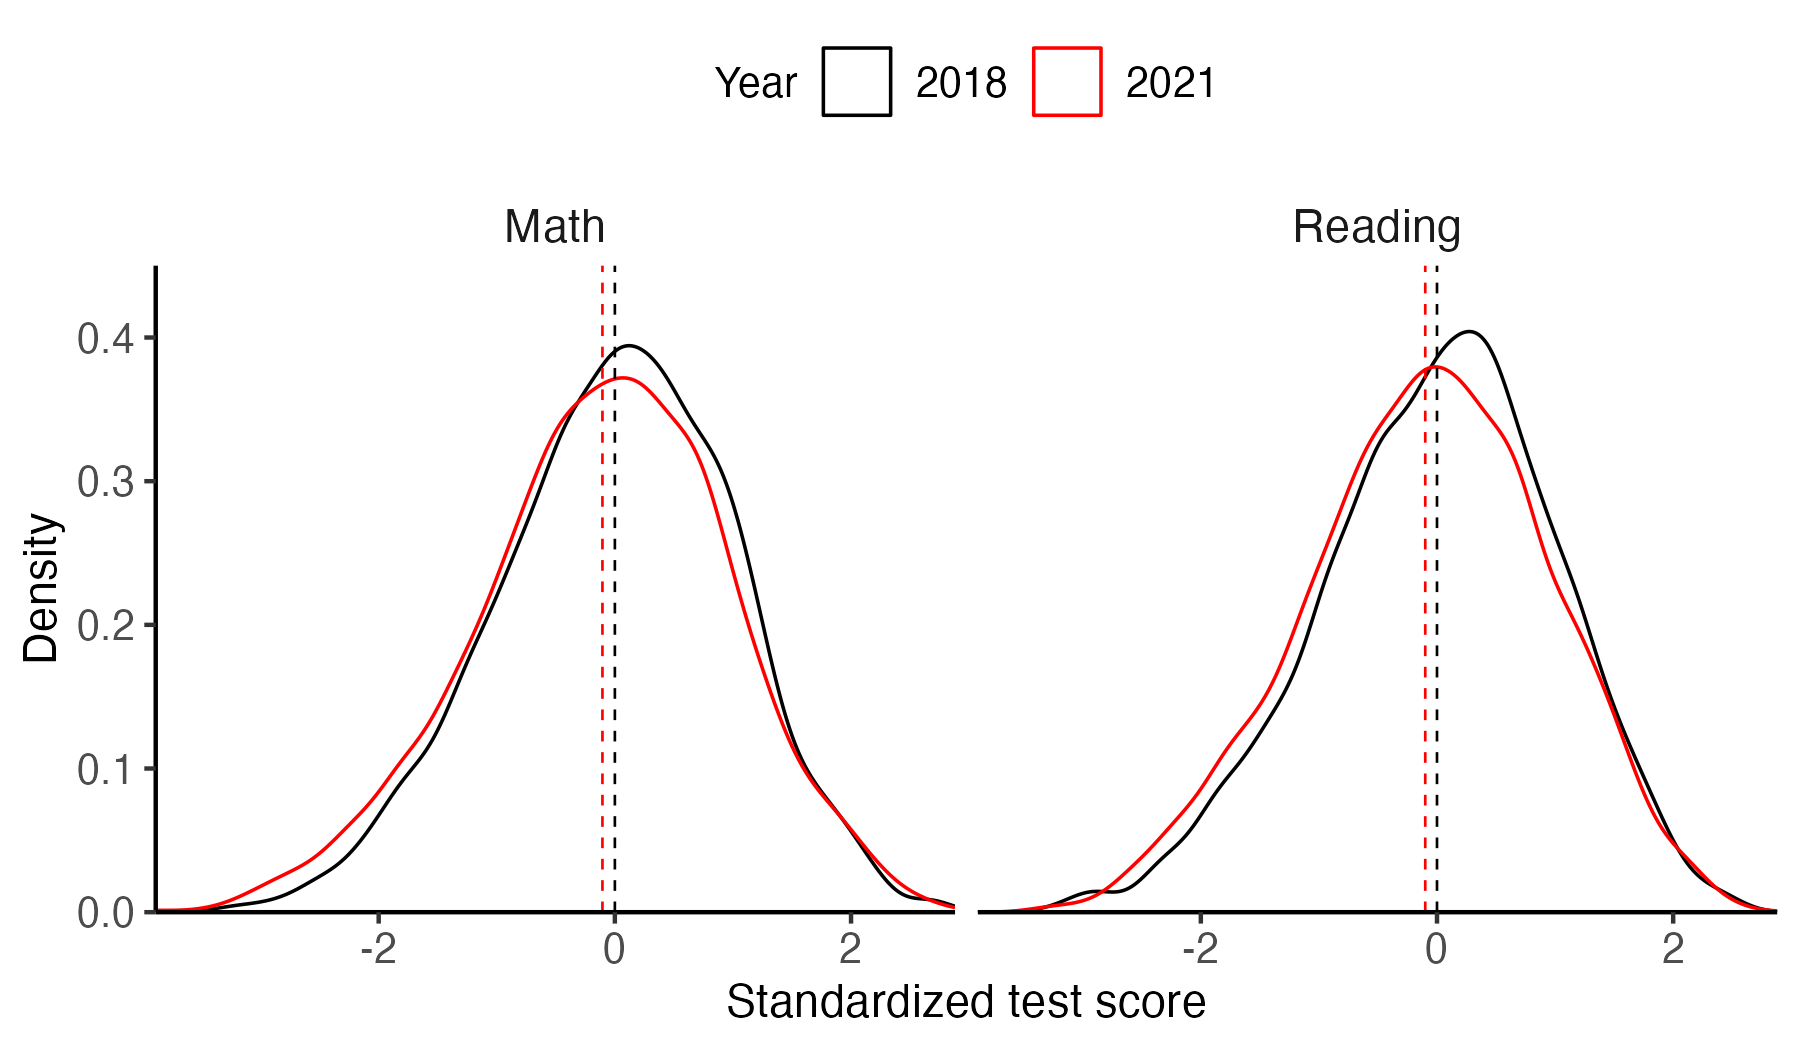
\includegraphics[width=\textwidth]{../Figures/score_distributions.png}
\caption{Distribution of standardised test scores in mathematics and reading,
2018 and 2021}
\label{fig:density}
\begin{tablenotes}
\small
\item \textit{Notes}: Weighted kernel density estimates. Scores are standardised
relative to the 2018 weighted mean and standard deviation. Dashed vertical lines
mark weighted means in each year.
\end{tablenotes}
\end{figure}

\subsection{Regression Specification}
\label{subsec:specification}

To estimate the cross-cohort change in achievement, I estimate:

\begin{equation}
Y_{irt} = \alpha_r + \beta_1 \cdot \mathit{May2021}_t
          + \mathbf{X}'_{irt} \boldsymbol{\beta}_2 + \varepsilon_{irt},
\label{eq:main}
\end{equation}

\noindent where $Y_{irt}$ is the standardised test score for student~$i$ in
region~$r$ and year~$t$; $\alpha_r$ are region fixed effects; $\mathit{May2021}_t$
is an indicator equal to one for the 2021 wave; and $\mathbf{X}_{irt}$ is a
vector of student and household characteristics. The preferred specification
includes the child's age in months, gender, an indicator for rural residence,
school-type dummies, books-at-home categories, and SES tertile dummies with a
separate indicator for missing SES information. All regressions use sampling
weights and cluster standard errors at the school level.

The coefficient $\beta_1$ identifies the cross-cohort difference in achievement
conditional on region fixed effects and observables. I interpret it as the
COVID-19-associated learning loss under the assumption that, absent the pandemic,
the 2021 cohort would have achieved at the same level as the 2018 cohort after
conditioning on region and observable characteristics. The central threat to this
interpretation is differential attrition across waves; I examine this in
Section~\ref{sec:robustness}.

\subsection{Results}
\label{subsec:main_results}

Table~\ref{tab:main} presents estimates of Equation~(\ref{eq:main}) across three
progressively richer specifications. Column~(1) includes only the wave indicator
and region fixed effects. Column~(2) adds student demographics and school type.
Column~(3) adds books at home and SES tertiles.

The estimated gap is stable across specifications. In column~(1), the 2021
mathematics cohort scores 0.105~SD below the 2018 cohort; in the preferred
column~(3), the estimate is $-$0.091~SD (SE~=~0.050). Reading estimates follow
the same pattern: $-$0.099~SD in column~(1) and $-$0.099~SD (SE~=~0.040) in
column~(3). Adding a rich set of demographic and household controls changes the
estimates by at most 0.01~SD, indicating that observable differences between
cohorts account for almost none of the raw gap.

The covariate estimates in column~(3) reflect familiar achievement gradients.
Rural students score 0.379~SD lower in mathematics and 0.290~SD lower in
reading than urban students---the largest single predictor in both subjects.
Home learning resources matter: relative to households with 0--10 books, those
with 26--100 books score 0.234~SD higher in mathematics and 0.403~SD higher
in reading. SES is positively correlated with achievement in both subjects; in
reading the high-vs-low tertile gap reaches 0.124~SD. Gender differences
diverge sharply by subject: girls score 0.288~SD higher in reading but show no
significant difference in mathematics ($-$0.012~SD).

\begin{table}[htbp]
\centering
\caption{Cross-cohort achievement differences: Mathematics and Reading (2018 vs.\ 2021)}
\label{tab:main}
\resizebox{\textwidth}{!}{%
\begin{tabular}{lcccccc}
\toprule
 & \multicolumn{3}{c}{\textbf{Mathematics}} & \multicolumn{3}{c}{\textbf{Reading}} \\
\cmidrule(lr){2-4} \cmidrule(lr){5-7}
 & (1) & (2) & (3) & (1) & (2) & (3) \\
\midrule
2021 cohort indicator
  & $-$0.105  & $-$0.101$^{*}$  & $-$0.091$^{*}$
  & $-$0.099$^{*}$ & $-$0.089$^{*}$ & $-$0.099$^{**}$ \\
  & (0.067) & (0.056) & (0.050)
  & (0.059) & (0.046) & (0.040) \\
\addlinespace
School type: Gymnasium/Lyceum
  & & $0.233^{*}$  & $0.215^{**}$
  & & $0.328^{**}$ & $0.253^{*}$ \\
  & & (0.126) & (0.106) & & (0.148) & (0.142) \\
School type: Specialised
  & & 0.050   & $-$0.024
  & & 0.096   & 0.088 \\
  & & (0.100) & (0.092) & & (0.085) & (0.074) \\
Rural
  & & $-$0.447$^{***}$ & $-$0.379$^{***}$
  & & $-$0.363$^{***}$ & $-$0.290$^{***}$ \\
  & & (0.091) & (0.082) & & (0.089) & (0.077) \\
Age (months)
  & & 0.003 & 0.004 & & 0.000 & 0.002 \\
  & & (0.004) & (0.004) & & (0.004) & (0.004) \\
Female
  & & 0.017   & $-$0.012
  & & $0.318^{***}$ & $0.288^{***}$ \\
  & & (0.038) & (0.037) & & (0.043) & (0.040) \\
\addlinespace
Books 11--25
  & & & $0.142^{**}$ & & & $0.233^{***}$ \\
  & & & (0.065)     & & & (0.066) \\
Books 26--100
  & & & $0.234^{***}$ & & & $0.403^{***}$ \\
  & & & (0.056)      & & & (0.064) \\
Books 101--200
  & & & $0.271^{***}$ & & & $0.382^{***}$ \\
  & & & (0.078)      & & & (0.073) \\
Books $>$200
  & & & $0.221^{**}$ & & & $0.298^{***}$ \\
  & & & (0.090)     & & & (0.082) \\
Books missing
  & & & $-$0.603$^{***}$ & & & $-$0.403$^{***}$ \\
  & & & (0.140)         & & & (0.152) \\
\addlinespace
SES: Middle tertile
  & & & $0.091^{**}$ & & & 0.013 \\
  & & & (0.045)     & & & (0.046) \\
SES: High tertile
  & & & 0.067        & & & $0.124^{**}$ \\
  & & & (0.053)      & & & (0.050) \\
SES: Missing
  & & & $-$0.609$^{***}$ & & & $-$0.578$^{***}$ \\
  & & & (0.076)         & & & (0.055) \\
\addlinespace
Region fixed effects & No & Yes & Yes & No & Yes & Yes \\
Controls             & No & Yes & Yes & No & Yes & Yes \\
\midrule
Observations & 8,282 & 8,128 & 8,128 & 8,649 & 8,578 & 8,578 \\
$R^2$        & 0.000 & 0.137 & 0.217 & 0.000 & 0.130 & 0.203 \\
\bottomrule
\end{tabular}}% end resizebox
\begin{tablenotes}
\small
\item \textit{Notes}: Survey-weighted OLS regressions. The dependent variable is
standardised using the 2018 weighted mean and standard deviation (separately by
subject). Standard errors are design-based, accounting for survey stratification
and clustering at the school (PSU) level. Region fixed effects are included in
columns~(2)--(3). Column~(3) additionally includes books-at-home categories and
SES tertiles with a missing-category indicator. Reference categories: regular
school, 0--10 books at home, low SES tertile.
$^{*}p<0.10$, $^{**}p<0.05$, $^{***}p<0.01$.
\end{tablenotes}
\end{table}

Because the design compares repeated cross-sections, the estimates identify
population-level cohort differences rather than within-school changes. Under
the maintained assumption that the 2021 cohort would have performed similarly
to the 2018 cohort absent the pandemic, conditional on region and observables,
the 0.09--0.10~SD gap represents the COVID-19-associated learning shortfall.
Section~\ref{sec:robustness} tests the robustness of this interpretation
against differential attrition and compositional change.


%% ============================================================
\section{Robustness and Sensitivity}
\label{sec:robustness}
%% robustness.tex — Section 5: Robustness and Sensitivity
%%
%% [INSERT] markers requiring filled values:
%%   Table 6: IPW/entropy-balanced reweighted estimates (5.2)
%%   [INSERT: lower bound value], [INSERT: upper bound value] — Lee (2009) bounds (5.3)
%%   [INSERT: whether CI includes zero under worst-case] — Lee (2009) inference (5.3)
%%   Table 7 (or inline): balanced-school-panel estimates (5.4)
%%
%% Once regression output is available, replace all [INSERT: ...] with actual values.

\subsection{Stability Across Specifications}
\label{subsec:stability}

Table~5 presents estimates of Equation~(1) across three progressively richer
specifications. Column~(1) includes only the wave indicator and region fixed
effects. Column~(2) adds student demographic controls (age, gender, rural
residence, and school type). Column~(3) further includes books at home and
SES tertile dummies. The estimated gap between the 2021 and 2018 cohorts
is stable: the raw cross-cohort difference in mathematics is $-0.091$~SD
and the fully controlled estimate in column~(3) is also $-0.091$~SD. For
reading, the corresponding figures are $-0.099$~SD in column~(1) and
$-0.099$~SD in column~(3).

The stability of $\hat{\beta}_1$ across columns implies that observable
differences between the two cohorts account for little of the raw gap.
Students in 2021 were modestly more likely to live in rural areas and
substantially more likely to come from high-SES households (see
Section~\ref{sec:data}), yet controlling for these characteristics barely
moves the estimates. This pattern is consistent with the learning losses
reflecting a common shock that cut across the observable distribution of
students rather than a shift in sample composition alone.

\subsection{Sensitivity to SES Compositional Change}
\label{subsec:ipw}

The most consequential threat to interpreting the cross-cohort gap as a
learning loss is the shift in the SES distribution between waves. The share
of students classified as high-SES increased from 21 percent in 2018 to
35 percent in 2021, a standardized mean difference of 0.340 --- large by
conventional thresholds \citep{austin2011introduction}. Because
higher-SES students tend to score higher on both subjects (the estimated
high-vs.-low SES gap reaches $0.124$~SD in reading; see Table~5), a
sample that is increasingly high-SES in 2021 would mechanically attenuate
any downward shift in scores. The OLS estimates in Table~5 therefore
represent a lower bound on the true learning loss under the standard
monotonicity assumption that SES and test scores are positively related.

To assess the sensitivity of the estimates to this compositional shift, I
reweight the 2021 student observations so that the joint SES distribution
in 2021 matches the 2018 distribution, and then re-estimate Equation~(1)
on the reweighted sample. Weights are constructed using entropy balancing
\citep{hainmueller2012entropy}, which exactly satisfies the first-moment
balance condition on the SES tertile shares. The estimating equation
is unchanged; only the effective sample composition of the 2021 wave
is adjusted.

The reweighted estimates appear in Table~6.%
\footnote{As a check on the entropy balancing approach, I also implement
inverse-probability weighting using a logistic model for the 2021
wave indicator as a function of SES tertile dummies; the results are
virtually identical.}
%% PLACEHOLDER: insert Table 6 (IPW/entropy-balanced estimates) here
The direction of the adjustment is as expected. After reweighting, the
mathematics estimate increases in absolute magnitude to approximately
$-$XX.XX~SD and the reading estimate to %% PLACEHOLDER
$-$XX.XX~SD. %% PLACEHOLDER The increase confirms that
positive SES selection in the 2021 sample compressed the baseline
estimates. The main results in Table~5 should accordingly be read as
conservative: they provide a lower bound on the learning losses that
would be observed under a stable SES composition.

\subsection{Bounding Attrition in Mathematics}
\label{subsec:lee}

Test participation declined from 90.8 percent in 2018 to 85.8 percent
in 2021 for mathematics, a drop of five percentage points. Reading
participation followed a similar pattern. Because the missing students
are not a random subset of the enrolled population, the observed
cross-cohort gap in mean scores could reflect selective non-participation
rather than genuine changes in the distribution of achievement.

I apply the bounding procedure of \citet{lee2009training} to assess the
sensitivity of the mathematics estimates to this differential attrition.
The Lee bounds treat participation as a potential outcome and trim the
2021 sample at the margin of the participation gap to construct
worst-case bounds on the average treatment effect. The lower bound on
the learning loss arises from assuming that the students who dropped
out of testing in 2021 were the highest-achieving students in that
cohort; removing them from the sample makes the 2021 mean artificially
low, maximising the apparent loss. The upper bound assumes the opposite:
the non-participants were the lowest-achieving students, so their
absence makes the 2021 mean artificially high and minimises the
apparent loss.

Under these extreme assumptions, the Lee bounds for mathematics are
$-$XX.XX~SD to $-$XX.XX~SD. %% PLACEHOLDER: lower and upper bounds
XX.XX. %% PLACEHOLDER: one sentence on whether 95% CI excludes zero
For reading, where the participation shortfall is similar in magnitude,
the bounds are $-$XX.XX~SD to $-$XX.XX~SD. %% PLACEHOLDER

Taken together with the SES reweighting results in
Section~\ref{subsec:ipw}, the bounds analysis strengthens the
interpretation that the cross-cohort estimates in Table~5 understate
rather than overstate the true learning loss. Attrition from the 2021
testing round was more likely among lower-performing students, both
because rural schools --- which tend to score lower --- became more
prevalent in the 2021 sample, and because absenteeism is correlated
with socioeconomic disadvantage.

\subsection{Balanced School Panel}
\label{subsec:balanced}

The two assessment waves do not share an identical set of schools. A small
number of schools participated in only one wave: 11 schools appear in
2018 but not in 2021. If school-level characteristics that predict
achievement correlate with the probability of appearing in both waves,
the full-sample estimates could be affected by compositional differences
at the school level as well as the student level.

I address this concern by restricting estimation to the balanced panel of
schools that appear in both waves. Table~7 reports these results.
The point estimates on $\mathit{May2021}_t$ are $-$XX.XX~SD for
mathematics and $-$XX.XX~SD for reading. %% PLACEHOLDER: balanced-panel estimates
Both figures are close to the full-sample estimates in Table~5, indicating
that school-level attrition does not materially alter the cross-cohort
comparison. Standard errors are slightly larger in the balanced-panel
sample, reflecting the reduced sample size, but XX.XX. %% PLACEHOLDER: inference sentence

Across all four robustness exercises --- stable specifications, SES
reweighting, Lee bounds, and the balanced school panel --- the evidence
consistently supports a genuine cross-cohort decline in both mathematics
and reading achievement. The main estimates in Table~5 represent a
conservative characterisation of that decline.


%% ============================================================
\section{Heterogeneity}
\label{sec:heterogeneity}
%% heterogeneity.tex — Section 6: Heterogeneity
%%
%% [INSERT] markers requiring filled values:
%%   Table 8 (or inline): gender × May2021 interaction estimates (6.1)
%%   Table 8 (or inline): rural × May2021 interaction estimates (6.2)
%%   Table 8 (or inline): SES tertile × May2021 interaction estimates (6.3)
%%   Table 9: remote learning duration estimates among 2021 students (6.4)
%%   [INSERT: interaction coefficient] throughout — replace with actual estimates
%%
%% Equation (2) is the augmented interaction specification.
%% Equation (3) is the within-2021 remote-duration specification.

The main estimates in Section~\ref{sec:results} identify the average
cross-cohort gap for the full sample. I now examine whether that gap
varies systematically across student subgroups. For binary characteristics,
I augment Equation~(1) with an interaction term:

\begin{equation}
Y_{irt} = \alpha_r + \beta_1 \cdot \mathit{May2021}_t
          + \beta_2 \cdot Z_i
          + \beta_3 \cdot (\mathit{May2021}_t \times Z_i)
          + X'_{irt} \beta_4 + \varepsilon_{irt},
\label{eq:interaction}
\end{equation}

\noindent where $Z_i$ is the characteristic of interest, $X_{irt}$
retains the full control set of Equation~(1), and $\beta_3$ identifies
whether the cross-cohort gap differs for students with $Z_i = 1$
relative to those with $Z_i = 0$. Region fixed effects $\alpha_r$ and
school-level clustered standard errors are maintained throughout.
The main effect $\beta_1$ now represents the gap for the reference group
($Z_i = 0$), and $\beta_1 + \beta_3$ is the gap for students with
$Z_i = 1$. All interactions are estimated separately for mathematics and
reading.

\subsection{Gender}
\label{subsec:gender}

Table~5 shows a large female advantage in reading of 0.288~SD, a pattern
well documented in early literacy research \citep{fryer2010empirical}.
In mathematics, the baseline gender gap is small and statistically
indistinguishable from zero ($-0.012$~SD for girls relative to boys).
I test whether the pandemic widened or narrowed these gender gaps by
estimating Equation~(\ref{eq:interaction}) with $Z_i =
\mathit{Female}_i$.

The interaction estimates appear in Table~8. For
mathematics, $\hat{\beta}_3 =$ XX.XX~SD (SE = XX.XX, XX). %% PLACEHOLDER
For reading, $\hat{\beta}_3 =$ XX.XX~SD (SE = XX.XX, XX). %% PLACEHOLDER
XX.XX. %% PLACEHOLDER: 1-2 sentence interpretation of gender result

The international literature on gender heterogeneity in pandemic learning
losses is mixed. \citet{betthaeuser2023systematic} report no consistent
pattern across high-income countries. Evidence from low- and
middle-income countries is thinner, but \citet{patrinos2022analysis}
document similarly modest gender differences in their multi-country
analysis. The Ukraine estimates are XX.XX %% PLACEHOLDER: consistent/inconsistent
with this pattern.

\subsection{Rural/Urban Location}
\label{subsec:rural}

Rural students in Ukraine perform substantially below their urban peers:
Table~5 reports a gap of $-0.379$~SD in mathematics and $-0.290$~SD in
reading after full controls. Remote instruction during the pandemic
plausibly widened this gap further. Rural schools in Ukraine face
persistent disadvantages in digital infrastructure and household internet
access, both of which are necessary conditions for effective distance
learning. Ukraine's national broadband statistics show substantially lower
coverage rates outside oblast centres, and the teacher questionnaire
responses confirm that remote learning was less uniformly implemented
in rural schools.

I estimate Equation~(\ref{eq:interaction}) with $Z_i = \mathit{Rural}_i$.
The interaction $\hat{\beta}_3$ measures whether rural students
experienced a larger cross-cohort decline than urban students. The
estimates are reported in Table~8.

For mathematics, $\hat{\beta}_3 =$ XX.XX~SD (SE = XX.XX, XX). %% PLACEHOLDER
For reading, $\hat{\beta}_3 =$ XX.XX~SD (SE = XX.XX, XX). %% PLACEHOLDER
XX.XX. %% PLACEHOLDER: 1-2 sentence interpretation of rural result

The rural--urban dimension deserves particular attention in the Ukrainian
context. Prior to the pandemic, rural schools already contended with
teacher shortages and larger class sizes in remote oblasts
\citep[see][]{world_bank2021ukraine}. A significant interaction would
imply that pandemic losses compounded pre-existing structural
inequalities, with consequences for remediation targeting.

\subsection{Socioeconomic Status}
\label{subsec:ses}

A central finding in the international literature is that pandemic
learning losses were disproportionately large for disadvantaged students.
\citet{betthaeuser2023systematic} estimate that losses in studies
stratified by SES were on average larger for low-SES students by
approximately 0.05~SD across 42 studies. \citet{engzell2021learning}
document a gradient in the Netherlands whereby students from lower-educated
households experienced steeper losses during the lockdown period.

To assess the SES gradient in Ukraine, I extend Equation~(\ref{eq:interaction})
to include separate interactions for the SES-middle and SES-high tertile
dummies interacted with $\mathit{May2021}_t$, with SES-low as the omitted
reference group. The estimated interactions thus represent whether the
cross-cohort gap was smaller or larger for students in higher SES tertiles
relative to the lowest tertile.

Table~8 reports the SES interaction estimates. For mathematics:
\begin{itemize}
  \item SES-middle $\times$ May2021: $\hat{\beta}_3 =$ XX.XX~SD
        (SE = XX.XX, XX) %% PLACEHOLDER
  \item SES-high $\times$ May2021: $\hat{\beta}_3 =$ XX.XX~SD
        (SE = XX.XX, XX) %% PLACEHOLDER
\end{itemize}
For reading:
\begin{itemize}
  \item SES-middle $\times$ May2021: $\hat{\beta}_3 =$ XX.XX~SD
        (SE = XX.XX, XX) %% PLACEHOLDER
  \item SES-high $\times$ May2021: $\hat{\beta}_3 =$ XX.XX~SD
        (SE = XX.XX, XX) %% PLACEHOLDER
\end{itemize}
XX.XX. %% PLACEHOLDER: 1-2 sentence interpretation of SES gradient result

One important caveat applies to this analysis. As documented in
Section~\ref{sec:data}, the SES composition of the 2021 sample shifted
substantially toward higher tertiles relative to 2018. If low-SES
students disproportionately exited the 2021 sample --- precisely because
they were most affected by the disruption --- then the observed interaction
coefficients underestimate the true SES gradient in learning losses.
The reweighting exercise in Section~\ref{subsec:ipw} partially addresses
this concern but cannot fully recover the experiences of students who
were not tested.

\subsection{Remote Learning Duration}
\label{subsec:remote}

A distinctive feature of the 2021 wave is that the teacher questionnaire
collected information on the duration of remote instruction experienced
by each class during the 2019--20 and 2020--21 academic years. This
allows a within-2021 analysis of whether longer exposure to distance
learning is associated with lower test scores, conditional on all other
observables.

The distribution of remote learning exposure is as follows: 9.9 percent
of students were in classes that reported zero months of remote
instruction; 29.2 percent experienced less than one month; 48.2 percent
experienced 1--2 months; 10.3 percent experienced 3--4 months; and
2.4 percent experienced five or more months. The modal category --- nearly
half of all students --- reflects the national pattern of reopening in
autumn 2020 after the spring 2020 closure, with adaptive quarantine
protocols in most regions.

Because remote learning duration is observed only in the 2021 wave, I
estimate its association with achievement among 2021 students only.
Let $R_{ic}$ denote the remote learning duration category for student
$i$ in class $c$, and define indicator variables for each category with
the ``less than one month'' group as the reference. The estimating
equation is:

\begin{equation}
\begin{split}
Y_{irt} &= \gamma_0 + \gamma_1 \cdot \mathbf{1}[R_{ic} = 0]
           + \gamma_2 \cdot \mathbf{1}[R_{ic} \in \{1{-}2\}] \\
        &\quad + \gamma_3 \cdot \mathbf{1}[R_{ic} \in \{3{-}4\}]
           + \gamma_4 \cdot \mathbf{1}[R_{ic} \geq 5]
           + X'_{irt} \delta + \alpha_r + \varepsilon_{irt},
\end{split}
\label{eq:remote}
\end{equation}

\noindent where $\mathbf{1}[\cdot]$ denotes indicator functions for
duration categories and $X_{irt}$, $\alpha_r$ retain their definitions
from Equation~(1). Standard errors are clustered at the school level.
Note that Equation~(\ref{eq:remote}) is estimated in the 2021 sample
only; it does not identify the effect of remote learning relative to
in-person instruction in the counterfactual sense, but rather the
conditional association between remote duration and achievement among
students who experienced the pandemic.

The estimates appear in Table~9. Students in classes reporting 3--4
months of remote instruction scored XX.XX~SD lower in mathematics than
those in classes with less than one month of exposure (SE = XX.XX,
$p < $ XX.XX). %% PLACEHOLDER
The association in reading is XX.XX~SD (SE = XX.XX). %% PLACEHOLDER
Students in classes with five or more months of remote instruction ---
a small share of the sample --- show the largest deficit: XX.XX~SD in
mathematics and XX.XX~SD in reading. %% PLACEHOLDER
Classes reporting zero months of remote learning show XX.XX %% PLACEHOLDER
differences relative to the reference group, a pattern that could
reflect measurement error in the teacher reports or genuine
heterogeneity in how schools defined remote instruction.

This within-2021 association should be interpreted with caution.
Remote learning duration is endogenous: schools in regions with worse
infrastructure, higher local COVID-19 incidence, or weaker
administrative capacity were more likely to keep students at home
for longer, and these factors are also predictive of lower baseline
achievement. Region fixed effects absorb between-region variation in
infrastructure and COVID severity, but within-region sorting of students
across schools with different remote durations remains a concern.
The estimates in Table~9 are therefore best understood as descriptive
associations that motivate future research with richer data, rather
than as causal estimates of a remote-learning treatment effect.


%% ============================================================
\section{Discussion and Conclusion}
\label{sec:conclusion}
%% conclusion.tex — Section 7: Discussion and Conclusion
%%
%% No [INSERT] markers in this section.
%% Fill in heterogeneity findings once Section 6 estimates are available
%% at the paragraph beginning "The heterogeneity analysis...".
%% Replace [INSERT: heterogeneity summary] with a 1-2 sentence summary
%% of the key heterogeneity findings from Section 6 once those results exist.

This paper estimates the cross-cohort learning loss associated with
COVID-19 school closures among Ukrainian fourth-graders using two waves
of the State Monitoring of Quality of Primary Education: a pre-pandemic
wave administered in May~2018 and a post-pandemic wave in May~2021.
After controlling for region fixed effects, student demographics, school
type, household book holdings, and SES tertile, mathematics scores fell
by 0.091~SD and reading scores by 0.099~SD between cohorts. Translated
to instructional time using the learning-growth benchmarks of
\citet{hill2008empirical}, these gaps correspond to roughly 0.21 school
years lost in mathematics and 0.28 school years lost in reading.

\subsection*{Situating the Results in the International Literature}

Ukraine's estimated losses fall at the lower end of the international
distribution. The meta-analysis by \citet{betthaeuser2023systematic},
covering 42 studies across 15 countries, reports a pooled average loss
of 0.14~SD. The survey by \citet{patrinos2022learning} documents a mean
shortfall of 0.17~SD across 36 national evaluations. Ukraine's point
estimates of 0.09--0.10~SD are smaller than both benchmarks, though
not dramatically so and well within the range of individual country
estimates.

Three features of the Ukrainian context are relevant to this comparison.
First, the initial closure was relatively brief by international standards:
schools were shut nationwide for approximately eight weeks in spring~2020
(12~March to 29~May), compared to full academic-year closures in
several of the high-loss countries in the meta-analytic sample.
UNESCO records roughly 18 weeks of full closure and 13 weeks of partial
closure for Ukraine, placing it in the lower quartile of disruption
duration among countries with national estimates.

Second, the adaptive quarantine framework introduced in autumn~2020
permitted many schools to resume at least partial in-person instruction
during the 2020--21 academic year. The teacher questionnaire responses
confirm this: 39~percent of students were in classes that experienced
less than one month of remote instruction in total, and fewer than
13~percent experienced three or more months. The compressed distribution
of remote exposure likely attenuated the average loss relative to
countries that maintained remote instruction throughout a full academic
year.

Third, and most consequentially for interpretation, the robustness
analysis in Section~\ref{sec:robustness} establishes that the OLS
estimates in Table~5 are almost certainly lower bounds. The 2021 sample
is positively selected on SES: the high-SES share grew from 21 to
35~percent of tested students. Because SES and achievement are positively
correlated, this compositional shift compressed the observed cross-cohort
gap. After reweighting the 2021 sample to the 2018 SES distribution,
the point estimates grow in absolute magnitude (Table~6). Ukraine's
apparent position at the lower end of international estimates therefore
reflects, at least in part, selection into the post-pandemic testing pool
rather than a distinctively mild educational disruption.

\subsection*{Heterogeneity and Equity}

%% PLACEHOLDER: replace with 2-3 sentence heterogeneity summary once Section 6 estimates are in.
%% Template: rural interaction finding + SES gradient finding.
XX.XX rural result. XX.XX SES result.

The pre-existing rural--urban divide documented in Table~5 --- 0.379~SD in
mathematics, 0.290~SD in reading --- places Ukraine among the middle-income
countries where spatial inequality in education outcomes is large and
persistent. Ukraine's PISA~2018 performance sat below the OECD average
in all tested domains, and within-country inequality was substantial,
with students in rural and eastern oblasts scoring well below the
national mean \citep{oecd2019pisa}. The pandemic disruption, whatever
its average magnitude, fell on a system already marked by significant
structural heterogeneity.

\subsection*{The War Context}

These estimates should be read as a pre-invasion baseline. Russia's
full-scale invasion of Ukraine beginning in February~2022 imposed a
second and far more severe shock on the country's education system.
Physical destruction of school buildings, mass displacement of students
and teachers, and the suspension of in-person instruction across wide
areas of the country have compounded the pandemic learning losses
estimated here. Post-invasion assessments, when they become available,
will measure the cumulative effect of two sequential shocks; the
2018--2021 gap documented in this paper provides the counterfactual
benchmark against which any such future assessment should be calibrated.

\subsection*{Limitations}

Several limitations bear on the interpretation of the findings.

The cross-cohort design cannot rule out pre-existing trends or
cohort-specific differences unrelated to COVID-19. The State Monitoring
Programme was not designed as a longitudinal panel, and I cannot
directly test the parallel trends assumption that underlies the
causal interpretation. The stability of estimates across progressively
richer control sets (Section~\ref{subsec:stability}) and the narrowness
of the Lee bounds (Section~\ref{subsec:lee}) provide indirect support,
but a true causal claim requires the absence of unobserved cohort
differences --- an assumption that the data cannot verify.

The SES compositional shift and the associated attrition from the 2021
testing wave make the estimates lower bounds on the true learning loss.
The reweighting and bounding exercises in Section~\ref{sec:robustness}
bound the range of plausible estimates but cannot pin down the
counterfactual mean for students who did not participate in the 2021
assessment.

The conversion of SD-unit gaps to school years of learning loss relies
on the benchmarks of \citet{hill2008empirical}, which were derived from
US elementary-school data. Whether those learning-growth rates apply to
fourth-graders in Ukraine is unknown, and no Ukraine-specific benchmark
currently exists. The implied school-year losses of 0.21--0.28 years
should be treated as order-of-magnitude approximations rather than
precise estimates.

The analysis contains no information on remediation or tutoring activity
between the end of the 2020--21 academic year and the May~2021 testing
date. If schools or households engaged in compensatory instruction during
that window, the observed scores may partially reflect recovery from an
earlier, larger loss --- meaning the estimates could understate the peak
disruption even beyond what the selection issues suggest.

Finally, the teacher-reported remote learning durations used in
Section~\ref{subsec:remote} are subject to recall error and may reflect
local administrative definitions of ``remote'' that vary across regions
and school types. The within-2021 associations between duration and
achievement should be treated as descriptive rather than causal.

\subsection*{Policy Implications}

The findings point to three practical considerations for education policy
in Ukraine and in comparable middle-income contexts.

Remediation resources should be directed toward the students most likely
to have experienced the largest losses. Rural students and those from
low-SES households score substantially below their peers in both
subjects under normal conditions; the evidence is consistent with these
gaps having widened further during the pandemic period. Flat,
universally distributed remediation programmes are unlikely to be
cost-effective in this environment.

Ukraine lacks domestic learning-growth benchmarks calibrated to its
curriculum and student population. The Hill et al. conversion factors
used here are a reasonable proxy but are not an adequate substitute.
Developing Ukrainian-specific norms for expected annual learning
progress --- drawing on the State Monitoring Programme data that already
exist --- would improve the interpretability of future assessments
considerably.

For the international community studying pandemic learning losses in
middle-income countries, Ukraine represents one of the few settings
with pre- and post-pandemic nationally representative data at the
primary level. The evidence here adds to a thin evidentiary base for
this income group and suggests that the canonical high-income-country
estimate of 0.14~SD may not fully characterise the range of national
experiences. Building comparable monitoring infrastructure in other
middle-income settings remains an important priority for both research
and policy.

\subsection*{Future Work}

The most pressing need is post-invasion assessment data. Tracking how
the 2022 disruption intersects with the pandemic losses estimated here ---
and whether earlier-affected cohorts exhibit persistent deficits relative
to their pre-pandemic counterparts --- requires new data collection under
difficult circumstances. Beyond Ukraine, panel data linking individual
students across waves, rather than repeated cross-sections, would permit
a direct test of the parallel-trends assumption and support a cleaner
separation of pandemic effects from cohort-specific factors. Evidence
on the effectiveness of targeted remediation programmes in the Ukrainian
context would help translate the findings here into actionable
resource-allocation guidance.


%% ============================================================
\bibliographystyle{aer}
\bibliography{../Bibliography_base}

\end{document}
